\documentclass[10 pt,usenames,dvipsnames, oneside]{article}
\usepackage{../../../modelo-ensino-medio}



\begin{document}

\begin{center}
  \begin{minipage}[l]{3cm}

\includegraphics[width=2cm]{logo}    
\end{minipage}\hfill
\begin{minipage}[r]{.8\textwidth}
 {\Large \scshape Atividade: Simulação do lançamento de uma moeda honesta}  
\end{minipage}
\end{center}
\vspace{.2cm}

\ifdefined\prof
%Habilidades da BNCC
\begin{objetivos}
\item a
\end{objetivos}

%Caixa do Para o Professor
\begin{goals}
%Objetivos específicos
\begin{enumerate}
\item Aplicar o modelo probabilístico equiprovável e usar tecnologia para realizar simulações de um fenômeno aleatório.
\end{enumerate}

\tcblower

%Orientações e sugestões
Essa atividade demanda o uso de tenologia. Sugere-se realizá-la em laboratório de informática. Sugere-se também que os alunos trabalhem em pequenos grupos de dois ou três alunos para cada computador disponível. As atividades poderão ser adaptadas de acordo com o conhecimento prévio dos estudantes. Nesssa atividade poderá ser usado o exemplo dado anteriormente, atribuindo um dos dois números para “cara”{} e, o outro, para “coroa”.
\end{goals}

\bigskip
\begin{center}
{\large \scshape Atividade}
\end{center}
\fi

Deseja-se simular o lançamento de uma moeda honesta uma grande quantidade de vezes e comparar a frequência relativa de caras com a probabilidade teórica 0,5 de obter uma cara quando a moeda é honesta.

\begin{figure}[H]
\centering

\noindent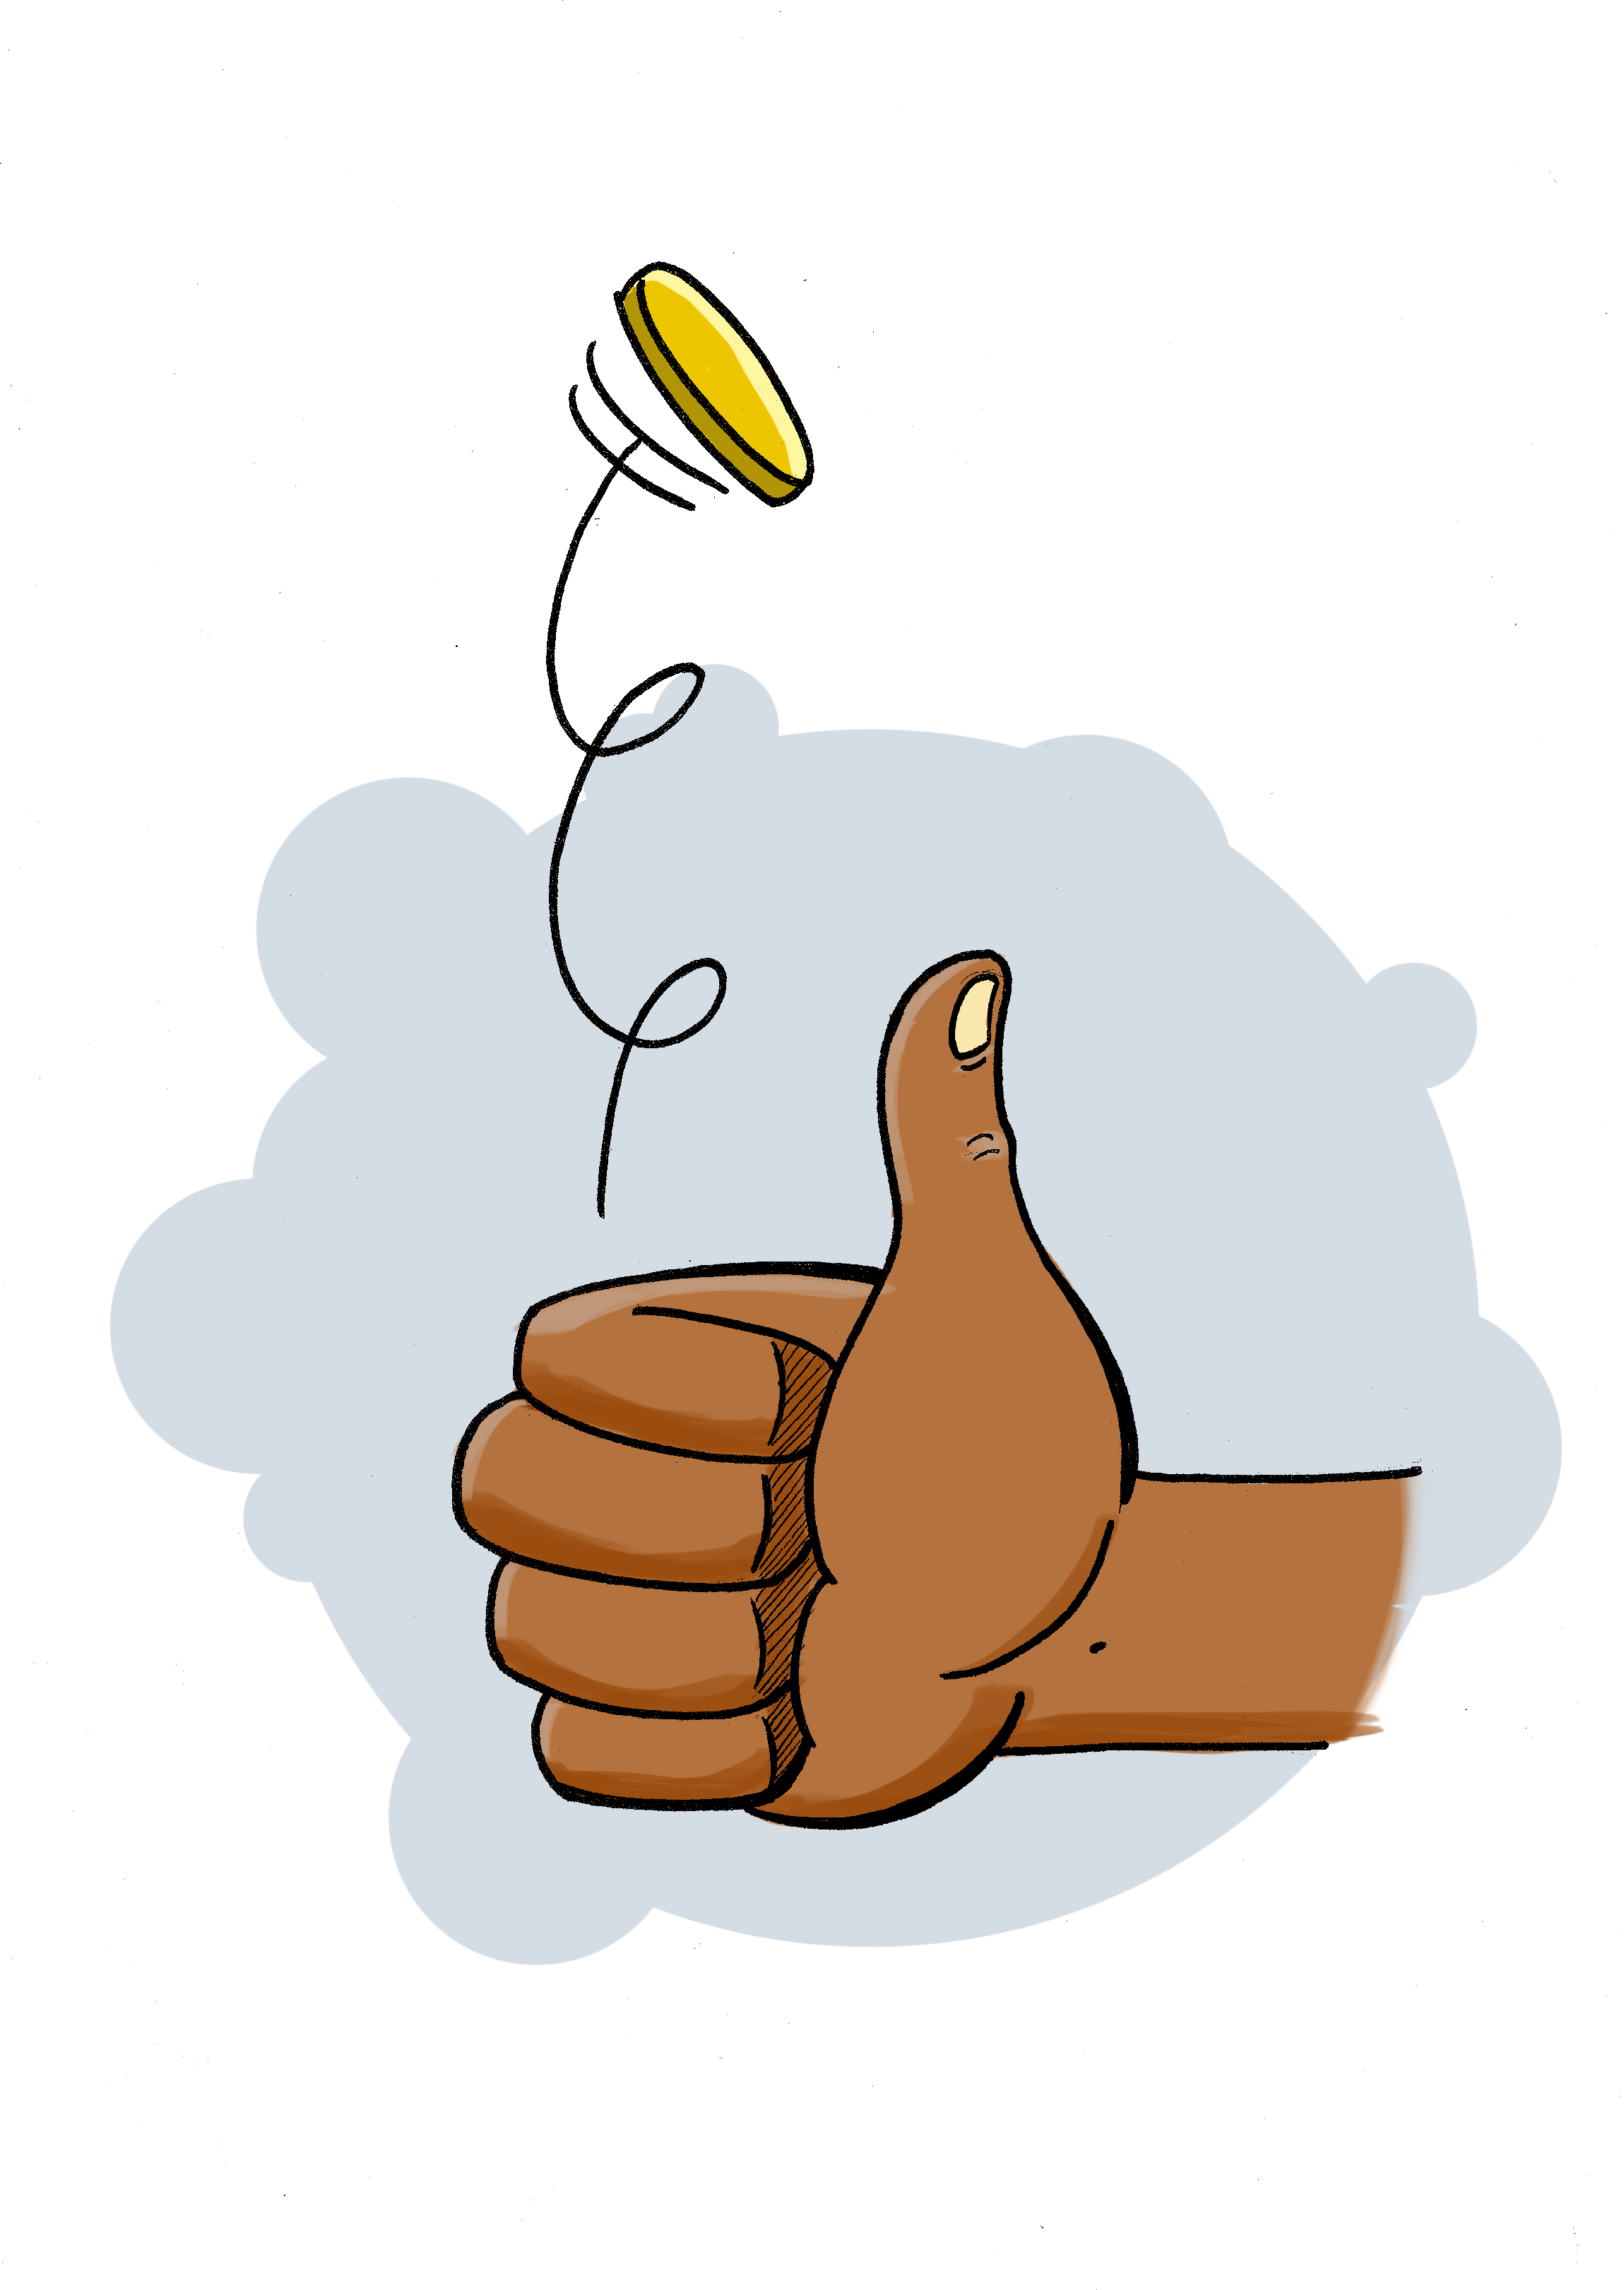
\includegraphics[width=125bp]{moeda.jpg}
\end{figure}
\begin{enumerate}
\item {} 
Usando o GeoGebra ou algum outro recurso tecnológico, simule 20 lançamentos da moeda e observe a quantidade de caras, calculando a frequência relativa.

\item {} 
Repita a simulação para 50, 100, 250 e 1000 lançamentos da moeda.

\clearpage
\item {} 
Complete o quadro a seguir e comente sobre os resultados obtidos.

\end{enumerate}

\begin{table}[H]
\centering
\begin{tabu} to \textwidth{|c|c|}
\hline
\thead
Número de Observações & Frequência relativa de caras \\
\hline
20 &\\
\hline
50 &\\
\hline
100 &\\
\hline
250 &\\
\hline
1000 &\\
\hline
\end{tabu}
\end{table}

\ifdefined\prof
\begin{solucao}

\begin{enumerate}
\item Você pode realizar a simulação usando a planilha do Geogebra e a função \textit{=NúmeroAleatório(1,2)} que irá gerar com probabilidades iguais ou o número $1$ ou o número $2$. Escolha um dos números para representar a ocorrência de cara e, o outro, para a ocorrência de coroa. Depois, arraste, copiando esta função para mais $19$ células, obtendo as $20$ simulações. Veja exemplo no início dessa seção. No GeoGebra ocorreram doze $1$’s (caras) e oito $2$’s (coroas) tal que a frequência relativa de caras observadas nessas 20 simulações foi $\frac{12}{20}=0{,}6$. É claro que as respostas irão variar, dependendo da simulação. Mas, espera-se que o número de $1$’s (caras) obtidos oscile em torno de $10$, pois a função produz os dois números com probabilidades iguais e geramos $20$ números.

\item Idem ao item anterior, só que agora os números de células a serem considerados na planilha são $50$, $100$, $250$ e $1000$, respectivamente.

\item No preenchimento da tabela você deverá perceber que a medida que o número de simulações é maior, a frequência relativa de caras se aproxima da probabilidade teórica de obter uma cara $(0{,}5)$. Se de fato o gerador de números aleatórios do programa que você está usando é bom, esse é o resultado esperado. Por exemplo, em uma simulação com o Geogebra foram observadas as seguintes frequências relativas de caras conforme o número de lançamentos:
\begin{table}[H]
\centering

\begin{tabular}{|f|f|}
\hline
$\tcolor{Número de Observações}$ & $\tcolor{Frequência relativa de 6}$ \\
\hline
20 & 0{,}45 \\
\hline
50 & 0{,}58 \\
\hline
100 & 0{,}51 \\
\hline
250 & 0{,}52 \\
\hline
1000 & 0{,}49 \\
\hline
\end{tabular}
\end{table}
\end{enumerate}

\end{solucao}
\fi

\end{document}